\pagebreak

\section{Requirements, Design \& Implementation}
In this section I discuss the requirements and design of the new component system introduced into \UH{} and give details about the new
implementation.

\subsection{Requirements}
I will first define the \textit{must-have} requirements, which need to be achieved to make the project a success.

As the code-base of \UH{} is already quite big and evolved it is not possible to create a design that requires a
complete rewrite of the code or which requires all the implementation work being done in one step. Therefore I aim at
creating a design that can be implemented in smaller steps and is compatible with the current code design.

I also aim at making it easy for content-creators to contribute new objects to the game and make it easy to edit
current object descriptions. The lack of an easily editable format can be considered of \UH{}'s major weaknesses
compared to other \OS{} games and has to be corrected. Therefore it is important to move away from the SQLite based
data-storage to a more humana readable and easily editable file based format. This file based format should be easy to
read and edit without special knowledge of computer programming.

It should be possible to add new components to entities by editing these files, changing the code must not be necessary.

An additional \textit{nice-to-have} requirement is that we do not add another dependency to the project, as in adding a
new library for the file format for example. This is not mandatory though and can be dropped if necessary. The usability
of the code and file format has a higher priority.

\paragraph{Gathered Requirements}\label{requirements}

\begin{enumerate}
    \item Porting the old code to the new structure should be possible in small steps
    \item Move object data from SQLite to a file based format
    \item The file format should be easy to understand by non-programmers
    \item Add/remove components by editing the files, not code
    \item No extra dependency (nice-to-have)
\end{enumerate}

\subsection{Design}
To ensure compatibility with the old inheritance based code, I will use a \textit{ComponentHolder} class, which manages all the
components an object has. This class can be included into any inheritance tree and thereby extending the current code
with the possibility of containing components. By using this approach I can slowly extract single classes from the code
and move them into components. A UML showing the planned implementation is shown in \figref{fig:codedesign}.

\begin{figure}[H]
\centering
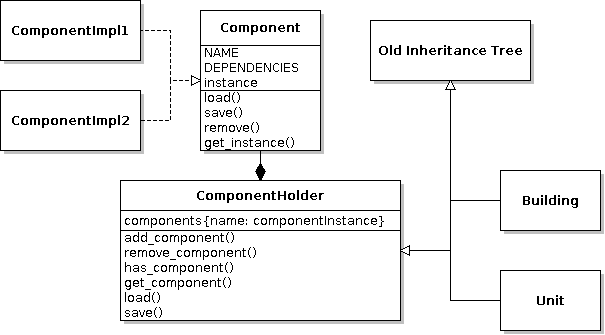
\includegraphics[width=0.9\textwidth]{pics/components_design}
\caption{The code design for the \textit{ComponentHolder} and \textit{Component} classes}
\label{fig:codedesign}
\end{figure}

A component should be a class to handle a specific task only and should be as independent
as possible from other components. Clearly a component can depend on other components being present, for example if I
decide to add a component that manages the production process, it will most likely depend on a component which manages
storage of items for this entity. These dependencies should be checked when the object is constructed to warn the
content creator if there are errors in this regard.
Each component has to be able to save and load its state without depending on any work being done by other components,
to ensure they are loosely coupled and easy to test.

\subsection{Implementation}
In this section I will discuss the details of the implementation.

\subsubsection{Data Format}
I decided to use YAML for the object description files, the requirements match and it avoids adding another
dependency to the project -- which was a \textit{nice-to-have} requirement (\secref{requirements}). The result of converting most of the data in the database to a YAML based file for each
object looks similar as \listref{uhyaml}. It contains all basic information needed for every building and a list of components
that are used by this specific building. As the conversion from an inheritance based approach to a component based
approach is only done in small steps, we have to specify the original base class for every object using the
\textit{baseclass} attribute.

\begin{lstlisting}[language=python,caption=A basic (shortened) building definition in YAML for \UH{}, label=uhyaml]
id: 24
name: Brickyard
baseclass: production.Refiner
size_x: 2
size_y: 4
inhabitants_max: 1
buildingcosts: {1: 500, 4: 6, 6: 1}
components:
- HealthComponent: {maxhealth: 1000}
- ProducerComponent:
    productionlines:
      33:
        produces:
        - [7, 1]
        consumes:
        - [21, -1]
        time: 15
- StorageComponent:
    inventory:
      SlotsStorage:
        slot_sizes: {21: 4, 7: 10}
\end{lstlisting}

\paragraph{Loading and Caching}
As loading YAML files is too slow to be repeated for every object creation in game, the data has to be cached after
reading it once. We use the abilities of Python to create a special type instance for every object. This type instance can
than be instantiated to a "normal" python object instance. It can be thought of as creating classes on the fly. We
create a lumberjack type for example, so for every new lumberjack in the game we can create a new object instance from
this type.
Since the data from the YAML file is only read once during type creation, we efficiently cache all the data in the
type instance for later use.

\subsubsection{Code Layout}
To achieve easy compatibility with the old inheritance based approach, a \textit{ComponentHolder} class has been
introduced, that manages a set of components. This class can be included into the normal hierarchy of any in-game object.

\paragraph{ComponentHolder}
The \textit{ComponentHolder} has a very basic interface:
\begin{itemize}
    \item initialize()
    \item add\_component()
    \item has\_component()
    \item get\_component()
    \item remove\_component()
    \item save()/load()/remove()
\end{itemize}
The add/has/get\_component() methods are pretty clear, they add \textit{Component}s to the \textit{ComponentHolder}, check if
they are available for this \textit{ComponentHolder} or return a specified \textit{Component}.

It is note-worthy that the \textit{ComponentHolder} contains an extra \textit{initialize()} method, which is separate from the
normal constructor. This method has to be called after instance creation on any class that inherits from the
\textit{ComponentHolder} class. This is a work-around for the problem that certain attributes, such as the game-engine's
visual instance, needed in the components are only ready after the entire constructor hierarchy has been executed to the
top. This will hopefully be repaired after everything has been moved to components, but for the moment this is a
necessary evil.

\paragraph{Component}
To represent a component the \textit{Component} class has been created. Each component should take care of a certain set
of functionality, which should be as independent as possible from any other code. Of course this is not always
achievable, as it soon becomes clear that special components will rely on the existence of other components. For example
a production component might rely on the presence of a storage component, with which it can work.

Each \textit{Component} has to implement the basic interface:
\begin{itemize}
    \item initialize()
    \item load()/save()
    \item remove()
    \item get\_instance() - class-method
\end{itemize}
As with the \textit{ComponentHolder} the \textit{Component} has to implement an \textit{initialize()} method, in which
all the setup should be done. This method is called automatically by the \textit{ComponentHolder}, so no special care
has to be taken here.

The \textit{load()}/\textit{save()} methods are called by the \textit{ComponentHolder} and should
implement loading and saving the components state into the given database. This should be done in a way, that the
component does not relay on any other part of the code to correctly restore its state on loading.

The \textit{get\_instance()} method is a class method, its purpose is to return an instance of the component, given data loaded
from the YAML file. For basic components the basic implementation is likely to suffice, it will pass in the dict of data
loaded from YAML as arguments to the class. For more sophisticated components this method might need to be
re-implemented. An example of this is the \textit{StorageComponent}.

Each component has to set the class's \textit{NAME} variable to unique string. Components that inherit from other
components can usually keep the name of the inherited class, as they are not used in the same \textit{ComponentHolder}
instance. Keeping the name the same, also ensures that if they implement similar functionality it is possible to call
\textit{get\_component()} with the parent class, and still receiving the correct implementation. This is used for example
for names. A \textit{NamedComponent} has been implemented. It handles giving names to objects. There are some special
implementations of this, for example the \textit{ShipNameComponent}, which uses special names designated for ships. If a
\textit{ShipNameComponent} component is present in the \textit{ComponentHolder} class and get\_component{NamedComponent}
is called, the \textit{ShipNameComponent} is returned, as they both use the same \textit{NAME} variable.

\subparagraph{Dependencies}
\textit{Components} can depend on other components to exist. For this every \textit{Component} class can use the
\textit{DEPENDENCIES} class variable. It is a list of \textit{Component} classes. The classes specified will be
initialized before the class that lists them as dependencies. 

The basic dependency resolution is done by implementing the \textit{\_\_lt\_\_()} (less than) method on the Component,
so that a list of \textit{Components} can be sorted by dependency order. This is of course a very basic form of
dependency resolution, which can't detect circular dependencies, etc. It should be good enough for this purpose and is very
simple and fast, as it uses python built-in \textit{sorted()} method.

\paragraph{Implementation Overview}
\begin{figure}[H]
\centering
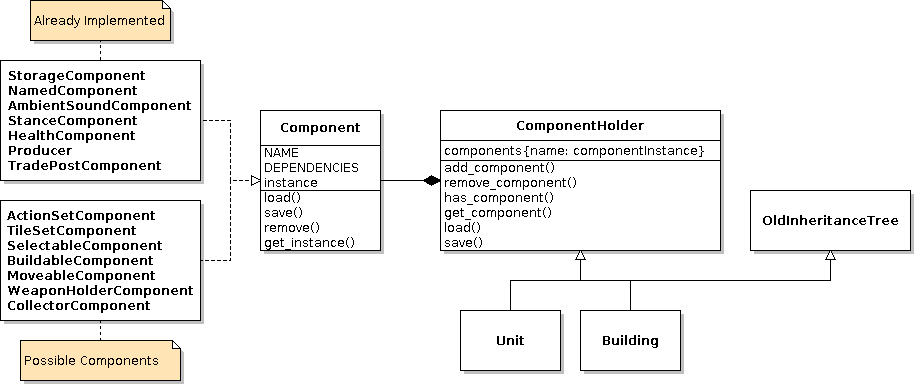
\includegraphics[width=0.9\textwidth]{pics/components_implemented}
\caption{UML diagram for the \textit{ComponentHolder} and \textit{Component} classes which were implemented}
\label{fig:codeimpl}
\end{figure}

\figref{fig:codeimpl} shows the basic layout of the implementation in a simple UML diagram. When compared to the first
settler class diagram in \figref{fig:settleruml} one can see that classes like \textit{Producer} have been pulled out of the
inheritance tree and are now used by composition with the \textit{ComponentHolder} instead.

\pagebreak

\subsection{Added Components}
Since the scope of the project is not big enough turn the \UH{} code-base into a completely component driven
architecture, only parts of the classes have been converted to \textit{Component}s yet. The following \textit{Component}
implementations have been made:
\begin{itemize}
    \item AmbientSoundComponent
    \item HealthComponent
    \item NamedComponent + Sub-classes
    \item StanceComponent
    \item StorageComponent
    \item TradePostComponent
    \item Producer
\end{itemize}

\paragraph{AmbientSoundComponent}
The \textit{AmbientSoundComponent} takes care of playing sounds in-game. It can position sounds at the current position
of an entity and saves a list of all the sounds an entity can play. The goal of this component is to collect all sound
handling code in one place. Since we do not have a lot of this code, this component was a good start together with the
\textit{NamedComponent}.

\paragraph{HealthComponent}
Together with the \textit{StanceComponent} this was one of the components that had been created during the project's
participation in \textit{Google Summer of Code 2011}. This was the first try of working on a component based system. I
did not make major changes to this component, other than fitting it into the new interface.

Its purpose is to provide a health counter for objects and handle everything that is connected with this, like drawing
life-bars.

\paragraph{NamedComponent + Sub-classes}
The \textit{NamedComponent} provides unique names for an object throughout one game. For this class several sub classes
exist, that provide different names. Namely these are:
\begin{itemize}
    \item \textit{ShipNameComponent}
    \item \textit{PirateShipNameComponent}
    \item \textit{SettlementNameComponent}
\end{itemize}

\paragraph{StanceComponent}
The \textit{StanceComponent} is used to set the combat stance of the object. It can be aggressive, defensive or neutral.
This Component was introduced during the \textit{Google Summer of Code 2011} as part of the combat system
implementation.

\paragraph{StorageComponent}
The \textit{StorageComponent} provides the entity with a sort of inventory where it can store different resources. This
is a fairly complex component, as it can use different storage implementations internally. For this reason this
component has to implement its own \textit{get\_instance()} method. An example markup for the \textit{StorageComponent}
using an inventory that can handle a fixed set of slots with specific sizes is given in \figref{storagyaml}.

\begin{lstlisting}[language=python,caption=YAML representation of the StorageComponent using a SlotStorage,
label=storagyaml]
- StorageComponent:
    inventory:
      SlotsStorage:
        slot_sizes: {28: 8, 5: 8}
\end{lstlisting}

\paragraph{TradePostComponent}
The \textit{TradePostComponent} adds trading functionality to the entity. This component handles selling and buying
resources from other players or the Free-Trader.

\paragraph{Producer}
This is most complex component in the game so far and I estimate it to stay this way, even if more components are added.
It manages the production of goods in the game, but using production lines. Since this is a very complex system it is
very bug-prone and extracting it into a single component and thereby removing it from the main hierarchy of buildings
was not easy. The code depended heavily on other classes being in the inheritance tree and debugging this was very
difficult and time-consuming.

The \textit{Producer} component greatly eases the changing and adjusting of production lines for the content creator, as
all information is now at one place. Using the old SQLite system, the content creator had to look at countless tables to
be able to get an overview of even a single production line. This has greatly improved. \listref{produceryaml} provides a short
example.

\begin{lstlisting}[language=python,caption=YAML representation of the Producer with two production lines,
label=produceryaml]
- ProducerComponent:
    productionlines:
      7:
        produces:
        - [10, 1]
        consumes:
        - [2, -1]
        time: 1
      47:
        produces:
        - [31, 1]
        consumes:
        - [30, -1]
        time: 1
\end{lstlisting}

\subsection{Converting the SQLite data to YAML}
Two methods were used when converting the SQLite data to YAML data: 
\begin{itemize}
    \item manual conversion
    \item converter script implemented in Python
\end{itemize}
The reason I used manual conversion is that \UH{} contains only very few units, for which a conversion script would not
have paid of in terms of total used time. I used the existing "print\_db\_data.py" to output relevant information to the
console and copied data straight from the SQLite file to create the new unit YAML definitions.

As there are over 40 building in \UH{} with many attributes, a different approach had to be taken. For this reason a
helper script was implemented in Python, which automatically converted the entire list of buildings into YAML building
definitions. This has the added benefit of avoiding syntax errors, as I let the YAML parser write the file instead of
writing it by hand. It also allowed testing different formats for the data, to find the best suited format. The
converter script is available in \textit{development/convert\_db\_to\_YAML.py}.

\subsection{Testing}
To ensure working code, three types of tests were used:
\begin{enumerate}
    \item Unit Test
    \item System Test
    \item Smoke Test
\end{enumerate}

\paragraph{Unit and System Tests}
\UH{} has a set of unit and system tests. Unit tests are basic tests for single classes to check their functionality.
System tests try to test the working of the entire game, instead of just a small function. It has a more general scope
to discover bugs in game logic.
After making the changes to the code, all tests have been repaired to work as expected. Also a few tests concerning the
new component system have been added. Together with the community I am working on extending the tests to cover more code
and to make sure my changes are stable before they are merged into the mainline of development.

\paragraph{Smoketests}
A smoke test describes a kind of test in which the goal is to run as much code of the system as possible and see if it
fails \cite{Mcconnell:1996:DBS:624614.625626}.

To emulate this, I used our artificial intelligence player. I started the game on 20 times the normal speed and
let 3 AI players play for a while. This helped me find a lot of bugs, especially in the beginning. As python is not
strictly typed, the interpreter discovers a lot of bugs, like missing attributes, only at run-time. Therefore it is
crucial to actually run as much game code as possible.

\section{Evaluation}
In this section I will evaluate the project and the result.

\subsection{Project}
The project was executed in an autonomous way, without much interaction of the professor or other mentors. The focus was
on mainly working with other people involved in \UH{} or other \OS{} games discussed in this work. This way it has a
direct impact on the work of \UH{} and might have led to some additional insights for members of other teams.

I believe the result matches the style of project execution, it had more emphasis on implementing the new
system than production many pages of documentation. A lot of time has been invested to implement a stable system that
can be used in the production mainline of development in \UH{}.

The plans for the implementation were worked on and discussed with the \UH{} team throughout the project and during the
weekly meetings\footnote{Meeting logs:
\url{http://meetings.christoph-egger.org/unknown-horizons/2011/unknown-horizons.2011-10-16-17.02.html}}\footnote{Meeting
logs 2: \url{http://meetings.christoph-egger.org/unknown-horizons/2011/unknown-horizons.2011-12-04-17.04.html}}. This
allowed me to identify weaknesses in my design and ensure that I have the same ideas, of how it should look, as the rest
of the team.

\subsection{Results}
This project provides two main results:
\begin{enumerate}
    \item Case-study of four existing systems to describe in-game entities
    \item Implementation of a new component system for \UH
\end{enumerate}

\paragraph{Case Study}
In the case study I have explained how the four project \UH{}, \BOW{}, \GLEST{} and \AD{} represent their objects as
in data format as well as in code. It provides insight for new projects on how a component based system can be designed
and on the quality of code-architecture in \OS{} games.

While the last part has not been explicitly discussed, it is clear that some thought on how to design these systems is
being put into the systems. Especially \AD{} provides a very cleanly designed system, designed for ease of development
and content creation with a very clear code structure.
It provides a purely component based system, making it the best designed of the four discussed projects under this point
of research.

\paragraph{Implementation}
The first lesson learned from this project is that refactoring the entire code of \UH{} into a component based system is
a lot of work, that if pursued further will require an enormous effort by the development team. Since it provides
great benefits to the code-quality, as in less coupling and thus better testability, it is likely that more work in this
area will be done.

Because of the amount of work this task requires, it was not possible to move the entire code to a
component based system in the time of this project and only a few proof of concept components have been implemented.

The implementation allows for an easier representation of entities outside the code, making it very interesting
for content creators, as they can now change the behavior of entities in the game in an easy way -- by just using a simple
text-editor. This has been enabled by using the YAML markup language to represent and save entity data. Simple
behavioral changes can be made by adding components to an entity and/or changing their attributes.

The use of YAML for entity description does not only allow using components in an easy manner, but also the changing of
data for entities, as this project involved moving most of the data from the main SQLite database into the YAML format.
This again enables easier work for the content creator.

I my opinion YAML is a better choice than \textit{XML}, because it is easier to read by humans and thus easier to handle
for non-programmers. Because we already use YAML for scenarios, it also means not adding another dependency and not
learning another markup language.

\paragraph{Settler Class}
To compare the old inheritance based class hierarchy, we compare the old UML tree given in \figref{fig:settleruml} with
the new version given in \figref{fig:settleruml2}:

\begin{figure}[!htb]
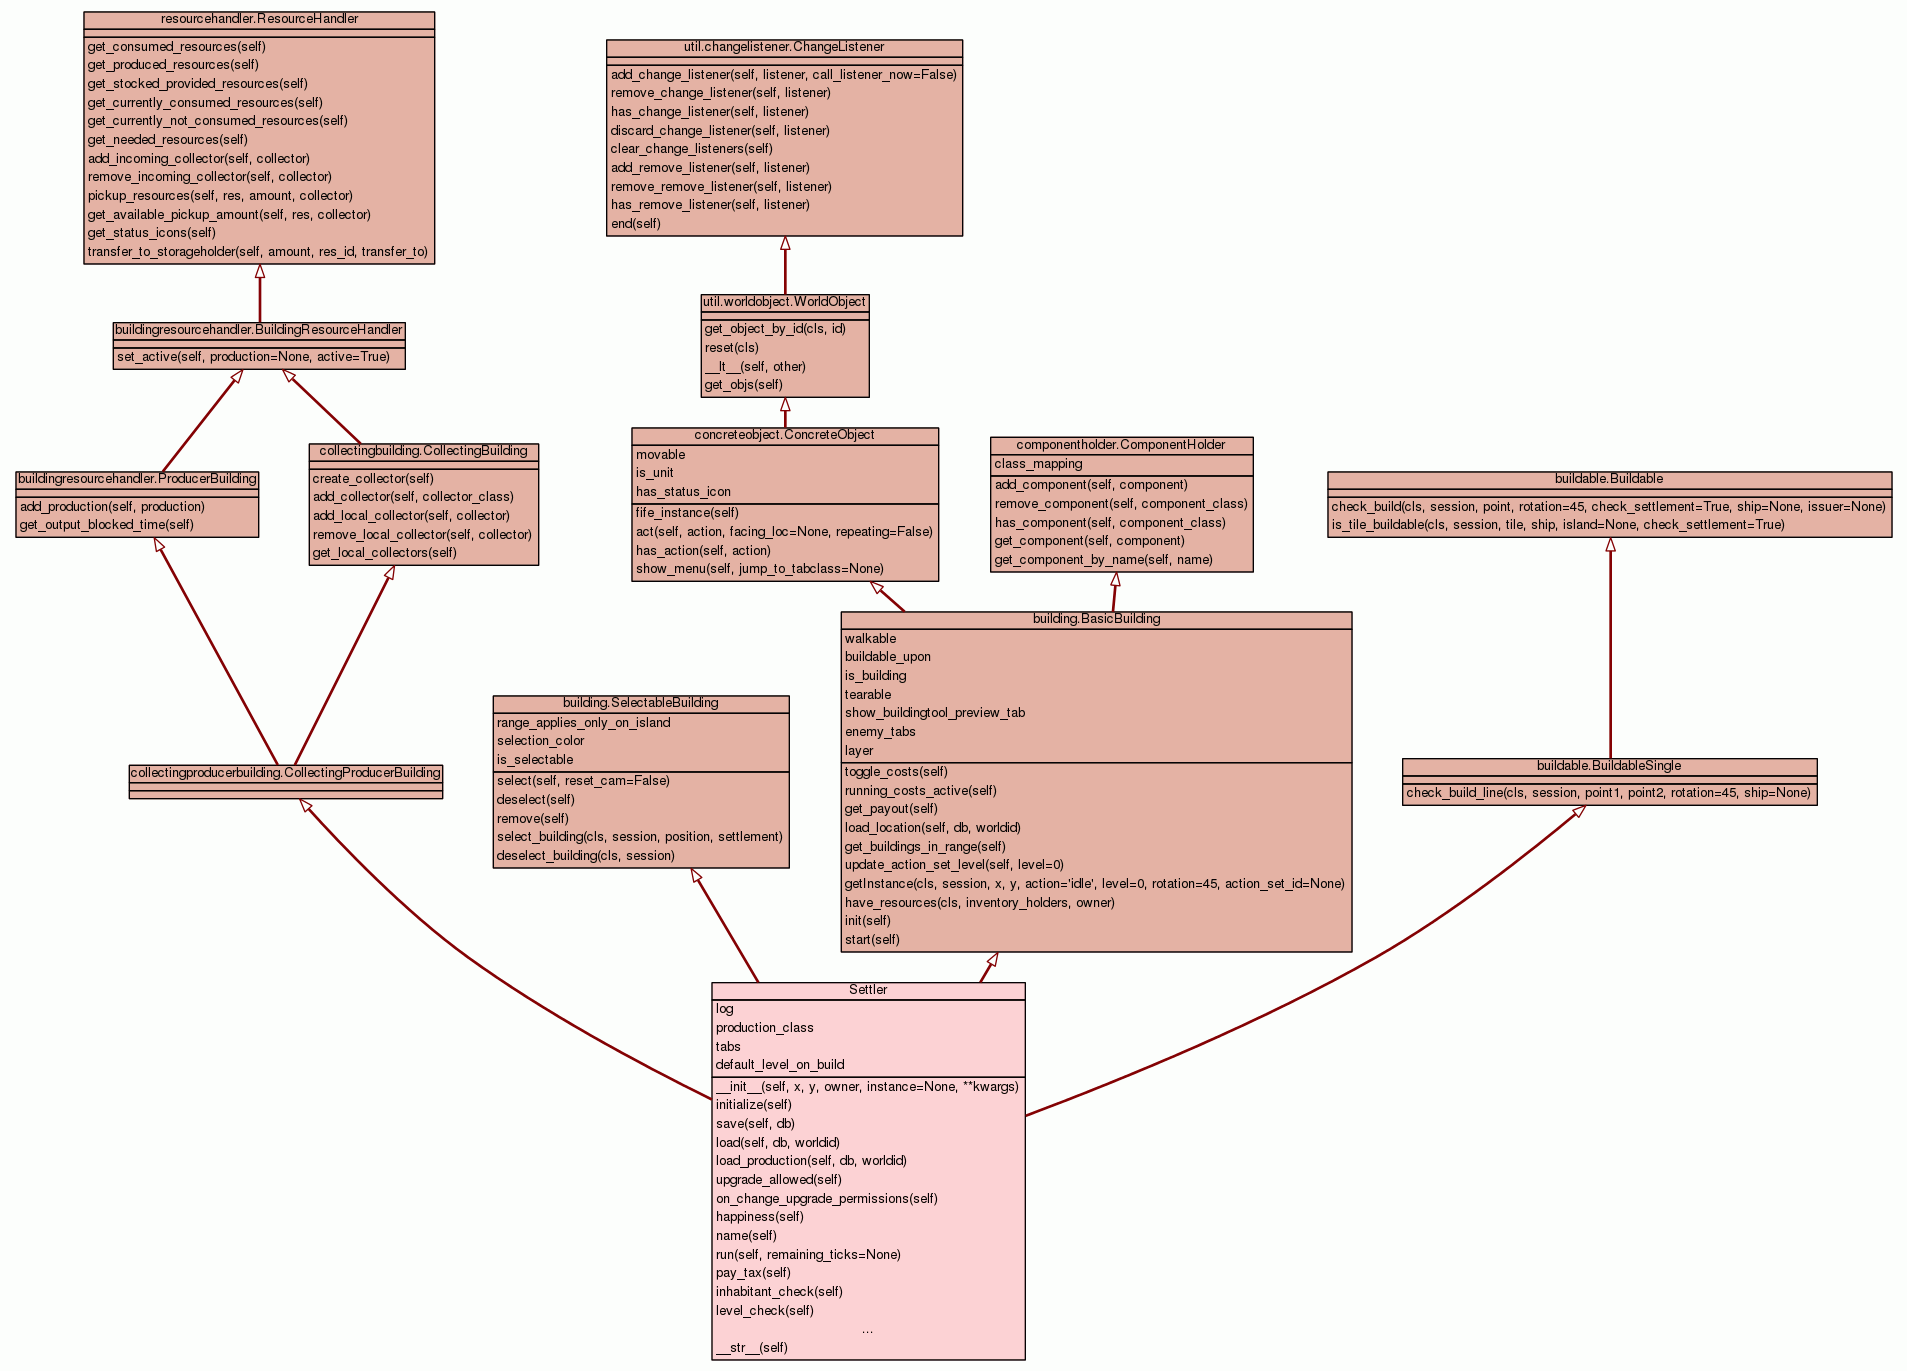
\includegraphics[angle=90,scale=0.35]{pics/settler_umlv}
\caption{Inheritance tree for the \textit{Settler} class in \UH{} after the addition of the ComponentHolder}
\label{fig:settleruml2}
\end{figure}

We removed the \textit{AmbientSound}, \textit{StorageHolder} and \textit{Producer} classes from the hierarchy, these are now used as components.
Not all created components are used in the \textit{Settler} class, so not all work is visible in this UML tree. However
it is clearly visible that the inheritance tree can be reduced in size by using components -- trimming it to a
small size still requires considerable work, as stated previously.

In my opinion especially the refactoring of the \textit{Producer} code into a \textit{Component} class brings great
benefits. The production code has been regarded as some of the most complex code in \UH{}, it is now much easier to
write tests for this part of the code, ensuring higher code quality on the long run.

\subsection{Methods}
Performing the research as a case-study seems to be a good idea, as there is hardly any dedicated literature available on
the topic of game architectures, specifically the area of entity description. Comparing \UH{} to other \OS{} projects
rather than commercial products makes sense, as, judging from experience, the man-power available matches a lot better than on commercial
projects. \OS{} projects usually don't have the time to create sophisticated tools, therefore it is crucial to rely on
simple methods for content creation.

The implementation created in this project can serve as a solid foundation for further work on the area of a component
based architecture. I believe that researching other projects first and then using the results gained from this study as
foundation lead to a nice solution for the scope of the \UH{} code base.
